\chapter{Background}

Skylab is built on top of Ruby on Rails, a well-known web development framework, with a great support from a large community, used widely in the industries by companies like Twitter, Groupon, Bloomberg, Airbnb and many more\cite{citation1}. There are many reasons why we have chosen Ruby on Rails. Firstly, Ruby is clean elegant and easy to read and this feature enables programmers to be more productive. Secondly, Ruby on Rails is adopting many advanced industrial conventions and this enables contributors to have good exposure to programming in the industry. What is more, scaffolding and many gems can significantly boost the productivity. Last but not least, Ruby on Rails community has a favor for open source contribution which aligns well with the open source nature of Skylab.

For the selection of database, we used PostgreSQL. Part of the reason is that it is open source and quite mature, with good drivers available in many languages\cite{citation2}. Besides, we need full ACID compliance for consistency of data and we do not need scalability in the foreseeable future. And PostgreSQL has recently added implementation for rich data structures such as JSON which would make development much easier\cite{citation3}.

Puma is the web server we have chosen for Skylab. Among Passenger, Unicorn, Rainbows! and Puma, Puma is considered to be fast and memory friendly according to on-line benchmarking\cite{citation4}. Puma is built for high-concurrency and speed and more and more developers to switching in Rails community\cite{citation5}.

Nginx has grown in popularity since its release due to its light-weight resource utilization and its ability to scale easily with low memory usage. It excels at serving static content quickly and is designed to pass dynamic requests off to other software that is better suited for those purposes\cite{citation6}. There are also some benchmarking results that indicate the superiority in Nginx handling concurrent access and low memory usage of Nginx\cite{citation7}. Therefore, Nginx has been chosen as our HTTP server.

\section{System design}

The basic MVC structure of Rails is shown in the figure below:
\begin{figure}[h]
\caption{Illustration of how MCV works in Rails}
\centering
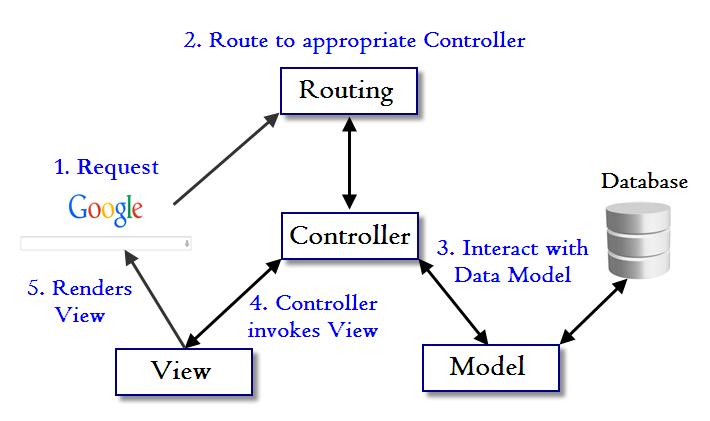
\includegraphics[width=0.7\textwidth]{MVC_Rails}
\end{figure}

\section{Development process}

To be continued